% $Header: /home/vedranm/bitbucket/beamer/solutions/conference-talks/conference-ornate-20min.en.tex,v 90e850259b8b 2007/01/28 20:48:30 tantau $
\documentclass{beamer}
\usepackage{amsmath,algorithm, algorithmic}
\usepackage{tikz}
\usetikzlibrary{shapes,arrows}
\usepackage[english]{babel}
% % or whatever

\usepackage[latin1]{inputenc}
% % or whatever

%\usepackage[T1]{fontenc}
% Or whatever. Note that the encoding and the font should match. If T1
% does not look nice, try deleting the line with the fontenc.
\usepackage{graphicx}
\usepackage{cmbright}
% This file is a solution template for:

% - Talk at a conference/colloquium.
% - Talk length is about 20min.
% - Style is ornate.



% Copyright 2004 by Till Tantau <tantau@users.sourceforge.net>.
%
% In principle, this file can be redistributed and/or modified under
% the terms of the GNU Public License, version 2.
%
% However, this file is supposed to be a template to be modified
% for your own needs. For this reason, if you use this file as a
% template and not specifically distribute it as part of a another
% package/program, I grant the extra permission to freely copy and
% modify this file as you see fit and even to delete this copyright
% notice. 
\mode<presentation>
{
  \usetheme{Amsterdam}
  %\usefonttheme{serif}
  % or ...

  \setbeamercovered{transparent}
  \beamertemplatenavigationsymbolsempty
  % or whatever (possibly just delete it)
}

\setbeamertemplate{footline}
{
  \leavevmode%
  \hbox{%
  \begin{beamercolorbox}[wd=.333333\paperwidth,ht=2.25ex,dp=1ex,center]{author in head/foot}%
    \usebeamerfont{author in head/foot}\insertshortauthor % Get rid of short institute next to name
  \end{beamercolorbox}%
  \begin{beamercolorbox}[wd=.333333\paperwidth,ht=2.25ex,dp=1ex,center]{title in head/foot}%
    \usebeamerfont{title in head/foot}\insertshorttitle
  \end{beamercolorbox}%
  \begin{beamercolorbox}[wd=.333333\paperwidth,ht=2.25ex,dp=1ex,right]{date in head/foot}%
    \usebeamerfont{date in head/foot}\insertshortdate{}\hspace*{2em}
    \insertframenumber{} / \inserttotalframenumber\hspace*{2ex} 
  \end{beamercolorbox}}%
  \vskip0pt%
}
\makeatother

\title[Photon Time Delay Estimation] % (optional, use only with long paper titles)
{Estimation of Time Delay in Gravitationally Lensed Photon Stream Pairs}

\author[Micha{\l} Staniaszek]{\large{Micha{\l} Staniaszek} \\ \scriptsize{Supervisor: Peter Ti\v{n}o}}
\institute[bham]{The University of Birmingham}

\setcounter{tocdepth}{1}

\date{\today}

% If you wish to uncover everything in a step-wise fashion, uncomment
% the following command: 

%\beamerdefaultoverlayspecification{<+->}

\begin{document}

\begin{frame}
  \titlepage
\end{frame}

\begin{frame}{Outline}
  \tableofcontents
  % You might wish to add the option [pausesections]
\end{frame}

\section{The Problem}

\subsection{Lensed Photon Streams}

\begin{frame}{A Basic Overview}
  \begin{itemize}
  \item<2-> Two rays of photons are emitted from a star or quasar
  \item<3-> Gravitational field of a massive object bends the rays
  \item<4-> Bent light means that we see two images of the source
  \item<5-> Capture arrival times of photons from each image (events)
  \item<6-> Stream $s_A$ arrives at time $t$, stream $s_B$ at $t + \Delta$
  \item<7-> \alert{We want to find $\Delta$}
  \end{itemize}
\end{frame}

\begin{frame}{What We Get}
  \begin{center}
      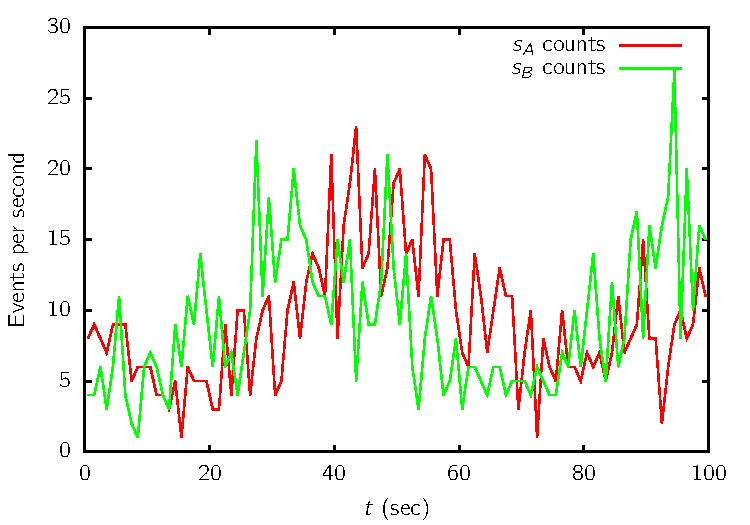
\includegraphics[width=4in]{twostreams_count}
  \end{center}
\end{frame}

\begin{frame}{What We Want}
  \begin{center}
      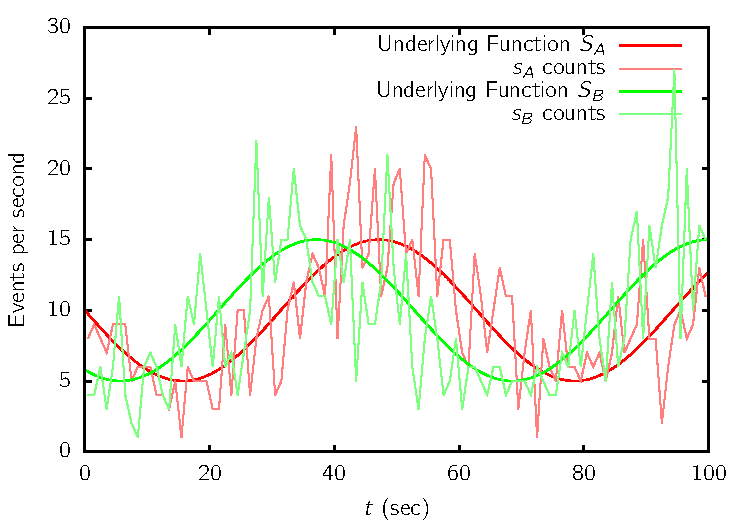
\includegraphics[width=4in]{twostreams_full}
  \end{center}
\end{frame}

\section{Why?}

\begin{frame}{What Can We Do With $\Delta$?}
  \begin{itemize}
  \item<2-> Estimate $H_o$
  \item<3-> Improve accuracy of stellar distance measurements
  \item<4-> Probe the nature of dark matter
  \item<5-> Detect extrasolar planets
  \item<6-> Measure mass distribution
  \item<7-> Many more proposed applications
  \end{itemize}
\end{frame}

\section{How?}

\subsection{Estimation Methods}

\begin{frame}{Previous Approaches}
  For estimation of the time delay from quasar Q0957+561, the following methods have been used:
  \begin{itemize}
  \item Structure-function based methods (PRH)
  \item Dispersion Spectra
  \item Cross correlation
  \end{itemize}
\end{frame}

\begin{frame}{How We Approach the Problem}
  Basic function estimation:
  \begin{itemize}
  \item Linear
  \item Piecewise linear
  \end{itemize}
  As a final goal:
  \begin{itemize}
  \item Model-based estimators with maximum likelihood
  \end{itemize}
\end{frame}

\begin{frame}{Implementation}
  The project will require implementation of:
  \begin{itemize}
  \item<2-> Photon event simulator (arrival time only)
  \item<3-> Linear and piecewise linear estimator
  \item<4-> Model based estimator
  \item<5-> A method for calculation of $\Delta$
  \end{itemize}
\end{frame}

\section{Progress}
\subsection{Current State}

\begin{frame}{What Have We Done So Far?}
  \begin{itemize}
  \item<2-> Photon arrival time simulation - \alert{complete}
  \item<3-> Linear estimator - \alert{complete}
  \item<4-> Piecewise estimator - in progress
  \end{itemize}
\end{frame}

\begin{frame}{Photon Simulation}
  We use a non-homogeneous poisson process (NHPP) to simulate arrival times.
  \begin{itemize}
  \item Rate parameter $\lambda$ is the expected number of arrivals per unit time
  \item Waiting time until the next event has an exponential distribution
  \item Time to next event in homogeneous process $t=-\frac{1}{\lambda}\ln(U)$
  \end{itemize}
\end{frame}

\begin{frame}{Poisson Generation Algorithm}
  \begin{algorithm}[H]
    \begin{algorithmic}[1]
      \REQUIRE $\lambda\geq \lambda(t), 0 \leq t \leq T$
      \STATE $E=\emptyset$, $t=0$, $T=\text{interval length}$
      \WHILE{$t<T$}
      \STATE Generate $U_1\sim U(0,1)$
      \STATE $t=t-\frac{1}{\lambda}\ln(U_1)$
      \STATE Generate $U_2\sim U(0,1)$, independent of $U_1$
      \IF{$U_2\leq\frac{\lambda(t)}{\lambda}$}
      \STATE $E \leftarrow t$
      \ENDIF
      \ENDWHILE
      \RETURN $E$
    \end{algorithmic}
    \caption{Simulating T Time Units of a NHPP by Thinning}
    \label{alg:seq}
  \end{algorithm}
\end{frame}

\begin{frame}{Linear Estimation}
  As a first step, attempt to estimate linear functions of the form $y=a+bx$ using Iterative Weighted Least Squares (IWLS)
  \begin{itemize}
  \item Extension of Optimum Least Squares (OLS) method.
  \item Find \[\min_{\alpha,\beta}\sum_{k=1}^{n}w_k(Y_k-[\alpha+\beta x])^2\]
  \item $\alpha$ and $\beta$ are estimators for $a$ and $b$, $w_k$ is the weight assigned to each value $Y_k$, which is the event count for the $k$th bin. $x$ is the midpoint of the sub-interval.
  \item Update weights at each iteration by using estimated values of $\lambda$ in each sub-interval.
  \end{itemize}
\end{frame}

\begin{frame}{Other Simple Methods}
  \begin{enumerate}
  \item Piecewise estimation
    \begin{itemize}
    \item Split the interval into sub-intervals and find an estimate for each one separately.
    \end{itemize}
  \item Baseline estimation
    \begin{itemize}
    \item Extension of the piecewise method. Find midpoint between two function estimates at breakpoints.
    \end{itemize}
  \end{enumerate}
\end{frame}

\begin{frame}{Piecewise Estimate Example}
  \begin{center}
      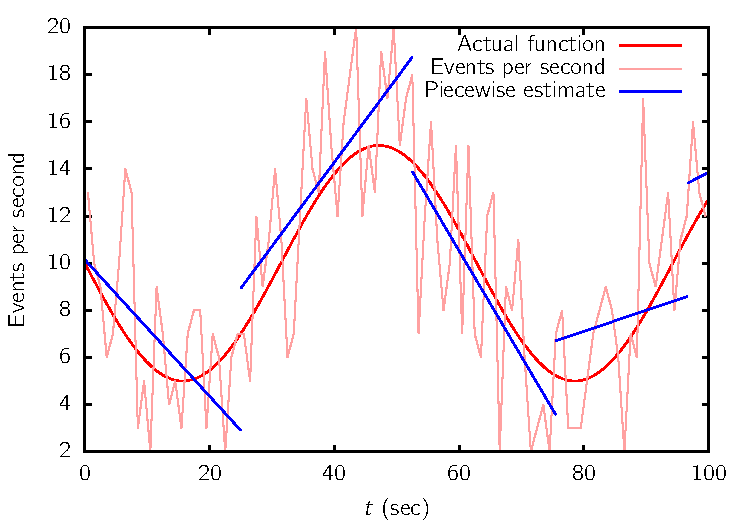
\includegraphics[width=4in]{piecewise}
  \end{center}
\end{frame}

\begin{frame}{Baseline Estimate vs Piecewise Estimate}
  \begin{center}
      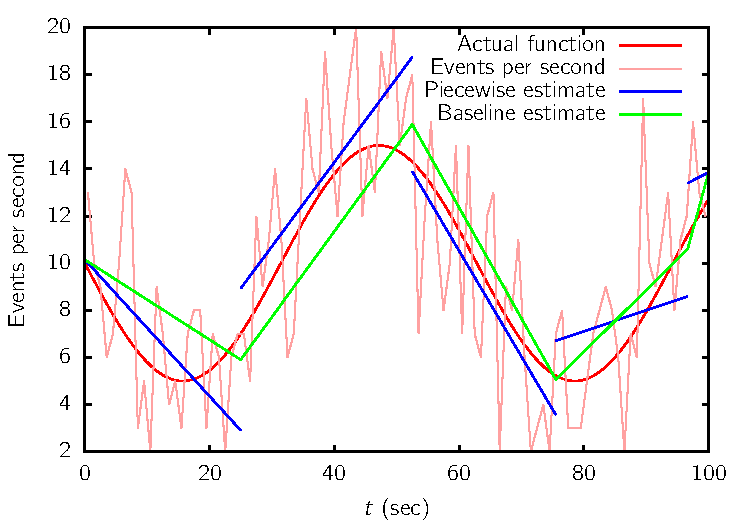
\includegraphics[width=4in]{baseline}
  \end{center}
\end{frame}

\begin{frame}{Model Based Estimation}
  \begin{itemize}
  \item Attempt to impose an explicit model on how $\lambda$ changes in time.
  \item Two streams of photons, $S_A$ and $S_B$ have models $\lambda_A(t)$ and $\lambda_B(t)$ respectively.
  \item If the two streams come from the same source, then $\lambda_B(t) = \lambda_A(t-\Delta)$, as both streams will have the same model.
  \item To calculate the time delay, we vary $\Delta$ and attempt to maximise the value of \[Pr(S_A,S_B|\lambda_A,\Delta)\]
  \end{itemize}
\end{frame}

\begin{frame}{Code Structure}
  % \pgfdeclarelayer{background}
  % \pgfdeclarelayer{foreground}
  % \pgfsetlayers{background,main,foreground}
  % \tikzstyle{sub}=[draw, fill=blue!20, text width=5em, 
  %   text centered, minimum height=1.8em]

  % \begin{tikzpicture}
    % % libs group
    % \node (math) at (6,2) [sub] {Math};
    % \node (gut) [sub, below of=math] {General};
    % \node (file) [sub, below of=gut] {File};
    % \node (lib) [below of=file] {Libraries};
    
    % \node (param) at (2,1.5) [sub] {Parameter server};
    % % generator group
    % \node (hom) at (0,0) [sub] {HPP};
    % \node (nhm) [sub, below of=hom] {NHPP};
    % \node (gen) [below of=nhm, font=\small] {Generators};
    % %\node (out) at (3,-1) [sub] {Output files};
    % % estimator group
    % \node (ln) at (4,0) [sub] {Linear};
    % \node (pc) [sub, below of=ln] {Piecewise};
    % \node (bl) [sub, below of=pc] {Baseline};
    % \node (est) [below of=bl, font=\small] {Estimators};
    % \begin{pgfonlayer}{background}
    %     % Estimator background
    %     \path (ln.north west)+(-0.2,0.2) node (a) {};
    %     \path (est.south -| ln.east)+(+0.2,-0.2) node (b) {};
    %     \path[fill=blue!10,rounded corners, draw=black!50, dashed]
    %         (a) rectangle (b);
    %     % generator background
    %     \path (hom.north west)+(-0.2,0.2) node (c) {};
    %     \path (gen.south -| hom.east)+(+0.2,-0.2) node (d) {};
    %     \path[fill=blue!10,rounded corners, draw=black!50, dashed]
    %         (c) rectangle (d);

    %     % path from param to est
    %     \path (ln.north)+(0,0.1) node (esttop){};    
    %     \draw [->,line width=1pt] (param.east) -| (esttop);
    %     % path from param to gen
    %     \path (hom.north)+(0,0.1) node (gentop){};    
    %     \draw [->,line width=1pt] (param.west) -| (gentop);
    %     % path gen->est
    %     \path (nhm.east)+(0.1,0) node (geneast){};
    %     \path (pc.west)+(-0.1,0) node (estwest){};
    %     \draw [->,line width=1pt] (geneast) -- (estwest);
    %     % paths from estimator bits
    %     \draw [->] (ln.south) -- (pc.north);
    %     \draw [->] (pc.south) -- (bl.north);
    %     % paths from gen bits
    %     \draw [->] (hom.south) -- (nhm.north);
    % \end{pgfonlayer}
    % \node (lib) at (0,0) [sub] {Libraries};
    % \node (est) at (1.5,-1) [sub] {Estimators};
    % \node (gen) at (-1.5,-1) [sub] {Generators};
    % \node (gra) at (4, -1) [sub] {Graphing scripts};
    % \draw [->] (lib.east) -| (est.north);
    % \draw [->] (lib.west) -| (gen.north);
    % \draw [->] (est.east) -- (gra.west);
%  \end{tikzpicture}
    The code is intended to be as modular as possible. Libraries are available to all modules and provide basic utilities that do not belong elsewhere. Current code is split as follows:
    \begin{itemize}
    \item Libraries (math, file, general)
    \item Generators
    \item Estimators
    \item Plotting scripts
    \end{itemize}
\end{frame}

\subsection{Projected Schedule}

\begin{frame}{Projected Schedule}
  \begin{itemize}
  \item  Over Christmas: 
    \begin{itemize}
    \item Complete piecewise estimators
    \item Code experiment harness, write unit tests, polish current code base
    \item Reading about ML, Latent Variable Models
    \item Implementing parts of ML estimator
    \end{itemize}
  \item End of January: Prototype ML estimator complete
  \item Mid February: ML estimator complete
  \item End of February: Estimation of $\Delta$
  \item Mid March: Experimentation complete
  \end{itemize}
\end{frame}


\section*{Summary}

\begin{frame}{Summary}

  % Keep the summary *very short*.
  \begin{itemize}
  \item
    We want to find the value of $\Delta$, the time delay between photon stream arrival times
  \item
    Currently have linear and piecewise linear estimators
  \item
    Final goal is to use a model-based estimator
  \end{itemize}
\end{frame}

\end{document}


